\section{Large Sample Confidence Intervals}
   The unbiased point estimates for $\mu,\; \rho,\; \mu_1 - \mu_0,\; \rho_1 - \rho_2$ all have near Normal distributions by the Central Limit Theorem.
   
   \nl Moreover, using
   $$Z = \frac{\that-\theta}{\sigma_{\that}}$$
   $Z$ is a pivotal quantity $N(0,1)$.

   \nnl For two-sided confidence intervals,
   $$\P{-Z_{\alpha/2} \leq Z \leq Z_{\alpha/2}} = 1 - \alpha$$
   
   \nl \begin{center}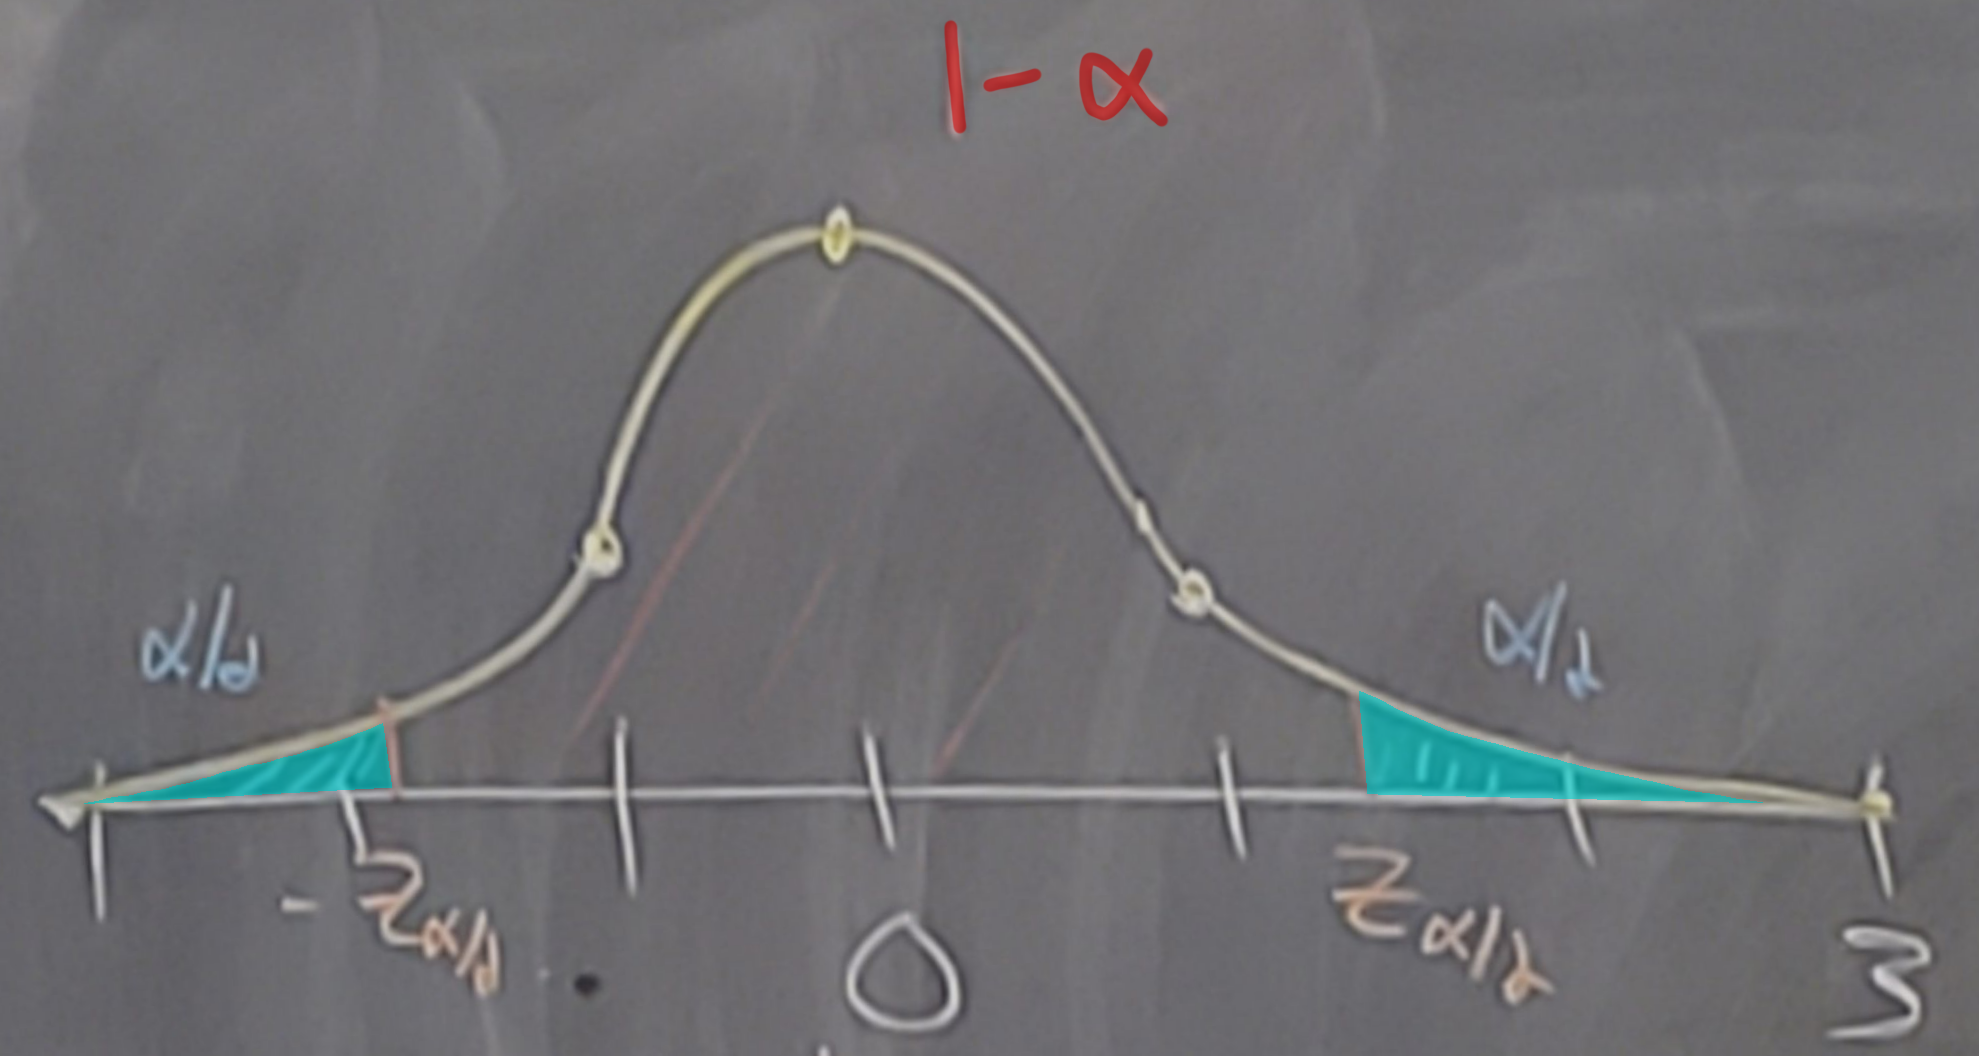
\includegraphics[width=6in]{alphaover2.png}\end{center}

   \nl Some common standard errors:
   \begin{align}
    90\% \text{ C.I. } \,& \Longrightarrow Z_{0.05} = 1.645\notag\\
    95\% \text{ C.I. } \, &\Longrightarrow Z_{0.025} = 1.960\notag\\
    99\% \text{ C.I. } \, &\Longrightarrow Z_{0.005} = 2.576\notag
   \end{align}
   Then
   $$-Z_{\alpha/2}  \leq Z \leq Z_{\alpha/2}$$
   $$-Z_{\alpha/2}  \leq \frac{\that-\theta}{\sigma_{\that}} \leq Z_{\alpha/2}$$
   $$-Z_{\alpha/2} \sigma_{\that}  \leq \that-\theta \leq Z_{\alpha/2} \sigma_{\that}$$
   $$-Z_{\alpha/2} \sigma_{\that} - \that \leq -\theta \leq Z_{\alpha/2} \sigma_{\that} - \that$$
   $$\underbrace{\that - Z_{\alpha/2} \sigma_{\that}}_{\that_L} \leq \theta \leq  \underbrace{\that + Z_{\alpha/2} \sigma_{\that}}_{\that_U}$$
           %green box around that with text 1-alpha confidence interval
           
    \noindent Of course, we don't know $\sigma_{\that}$ exactly. For \say{large} samples, we can use $\sigma_{\that} \approx S_{\that}$.
    
    \example*
    $$\Xbar = 19.07 \hspace{1in} S^2 = 10.60 \hspace{.75in}\text{with}\hspace{0.25in} n = 32$$
    \textit{Recall:} For \say{large} samples ($n \geq 30$), $\Xbar$ nearly distributed by $N(\mu, \sigma^2_{\Xbar}) \approx N(\mu, \frac{10.60}{0.32})$.
    \\For a $95\%$ CI for $\mu$,
    $$\sigma_{\Xbar} \approx \sqrt{\frac{10.60}{0.32}} \approx 0.576$$
    Here, $\alpha = 0.05$ and $\frac{\alpha}{2} = 0.025$. So $\Xbar \pm Z_{0.025} \sigma_{\Xbar}$, thus
    $$19.07 \pm (1.96)(0.576)$$
    $$\Rightarrow 19.07 \pm 1.128 \quad \text{or} \quad (17.94,\, 20.20)$$

    \disc* Differences in population proportions.

    \nl Estimating $p_1 - p_2$ by $\phat_1 - \phat_2$ for samples of size $n_1$ and $n_2$ respectively.
    \begin{align}
        \that\,\pm\, Z_{\alpha / 2} \sigma_{\that} &\quad\implies\quad \phat_1 - \phat_2 \,\pm\, Z_{\alpha/2} \sqrt{\sigma_{\phat_1}^2 + \sigma_{\phat_2}^2 } \notag\\
        &\quad\implies\quad \phat_1 - \phat_2 \,\pm\, Z_{\alpha/2} \underbrace{\sqrt{\frac{p_1q_1}{n_1}+\frac{p_2q_2}{n_2}}}_{\substack{\text{Depends on the} \\ \text{unknowns } p_1,\; p_2}}\notag
    \end{align}

    
    \nl Two standard fixes:
    \begin{enumerate}[label=\textcircled{\raisebox{-1pt}{\arabic*}}]
        \item $pq = p(1-p) \leq 1/4$\\
            Easy to show by calculus. Yields a \say{max} error via
            $$\sqrt{\over{4n_1}+\over{4_n2}}.$$
            However, in practice we use \cir{2} as smaller confidence intervals are desirable.
        
            \vspace{0.35in}
            \item When $n_i$ is large enough, we can use $\phat_1$ for $p_i$.
        
        \nl The $1-\alpha$ confidence interval is
        $$\phat_1-\phat_2 \,\pm\, Z_{\alpha/2}\sqrt{ \frac{\phat_1(1-\phat_1)}{n_1}   \, + \, \frac{\phat_2(1-\phat_2)}{n_2}  } $$
    \end{enumerate}
           